\documentclass{beamer}

\usepackage[utf8]{inputenc}
\usepackage{color}
\usepackage{amsfonts}	% Real

\usepackage{booktabs} % eleganckie tabelki


\usetheme{boxes}      % Wybór tematu wyglądu, gdy chcemy inny
%\usecolortheme{rose}   % Wybór tematu kolorystycznego, j.w.

%Konfiguracja dla pakietu hyperref:
\hypersetup{
  unicode=true,           % włączenie wyświetlania pliterek w zakładkach
%  pdfpagemode=FullScreen, % włączenie trybu pełnoekranowanego
  pdfsubject=Graph Neural Networks,      % temat prezentacji
  pdfkeywords={gnn, graph neural network, graph, classification} % slowa kluczowe
}

%% Dane do strony tytułowej
\author{Aleksy Barcz}
\title{Graph Neural Networks for crystal structures}
\date{\today}
\institute{Warsaw University of Technology}

\setbeamercovered{transparent}

\begin{document}
\frame{\titlepage}

\begin{frame}
\frametitle{Graph-oriented neural networks}
\begin{columns}
	\begin{column}{0.66\textwidth}
		\begin{itemize}
			\item Process information about graph structure directly
			\item Build meaningful representation
			\item Capable of classification and regression
			\item Based on feed-forward neural networks
		\end{itemize}
	\end{column}
	\begin{column}{0.34\textwidth}
		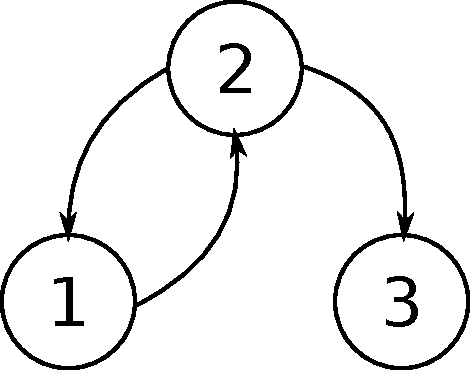
\includegraphics[scale=0.4]{img/graph}
	\end{column}
\end{columns}
\end{frame}

\begin{frame}
\frametitle{Applications of graph-oriented neural networks}
\begin{itemize}
	\item Drug design
	\item Prediction of fuel compounds properties
	\item Object detection in 2D images
	\item Document mining
\end{itemize}
\end{frame}

\begin{frame}
\frametitle{GNN - encoding network}
\begin{center}
	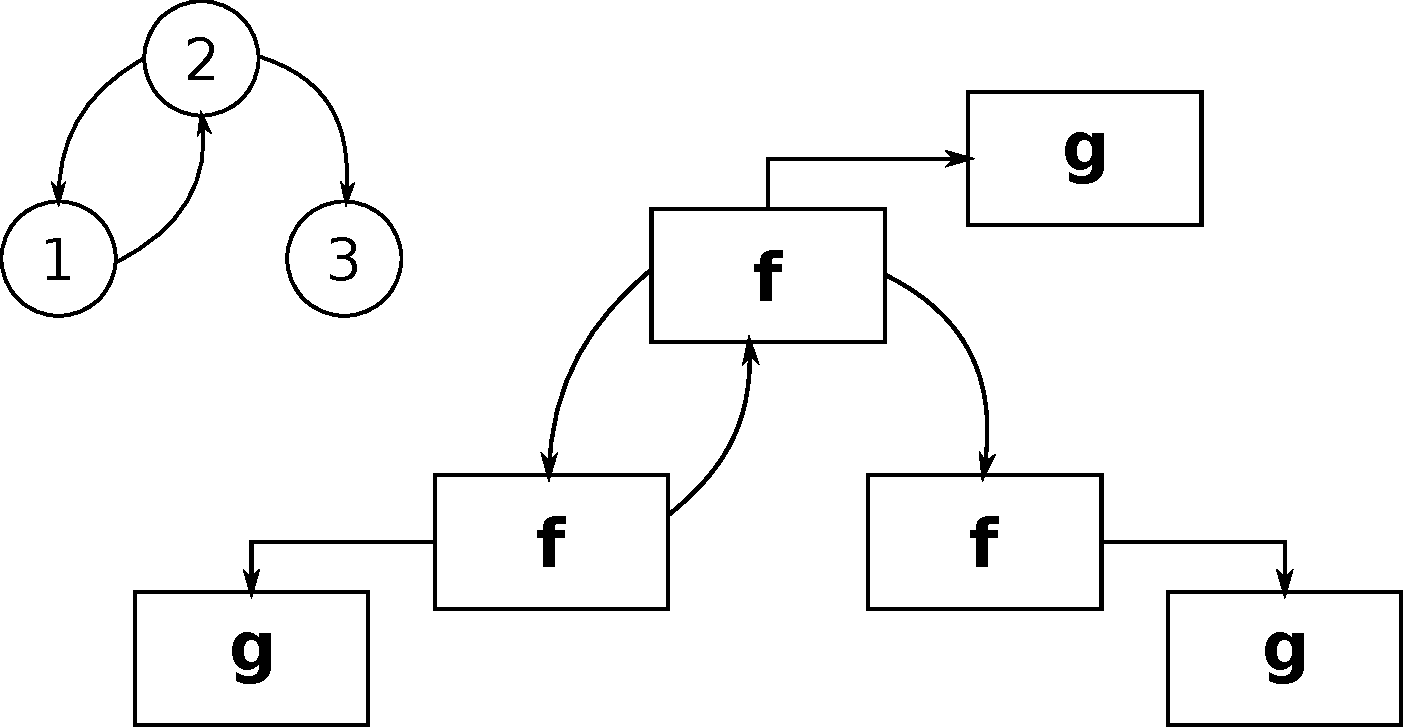
\includegraphics[scale=0.4]{img/encodinginc}
\end{center}
\begin{itemize}
	\item Building node representation: $x_n = f(...)$
	\item Node classification: $o_n = g(x_n)$
\end{itemize}
\end{frame}

\begin{frame}
\frametitle{Example - single substitution, tetragonal I cells}
\begin{columns}
	\begin{column}{0.34\textwidth}
		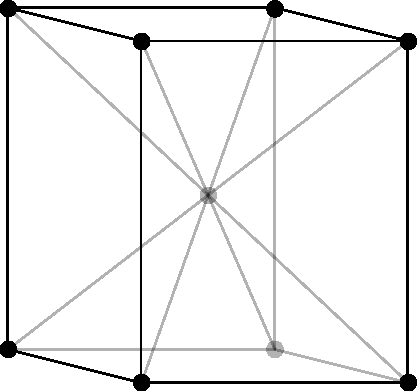
\includegraphics[scale=0.4]{img/tetragonal-I}
	\end{column}
	\begin{column}{0.66\textwidth}

\begin{table}[h!]
\begin{center}
\caption{Substitution existence}
\begin{tabular}{llll}
\hline\noalign{\smallskip}
 & accuracy & precision & recall\\
\noalign{\smallskip}
\hline
\noalign{\smallskip}
training set & 96.00\% &  96.00\% & 96.00\% \\
test set & 94.92\% & 95.29\% & 94.51\% \\
\hline
\label{tab:subst}
\end{tabular}
\end{center}
\end{table}

\begin{table}[h!]
\begin{center}
\caption{Substitution location difference}
\begin{tabular}{llll}
\hline\noalign{\smallskip}
 & accuracy & precision & recall\\
\noalign{\smallskip}
\hline
\noalign{\smallskip}
training set & 96.33\% &  94.26\% & 98.66\% \\
test set & 95.07\% & 92.05\% & 98.66\% \\
\hline
\label{tab:substloc}
\end{tabular}
\end{center}
\end{table}

	\end{column}
\end{columns}

\end{frame}

\begin{frame}
\frametitle{Application to Si defects - possibilities}
\begin{center}
	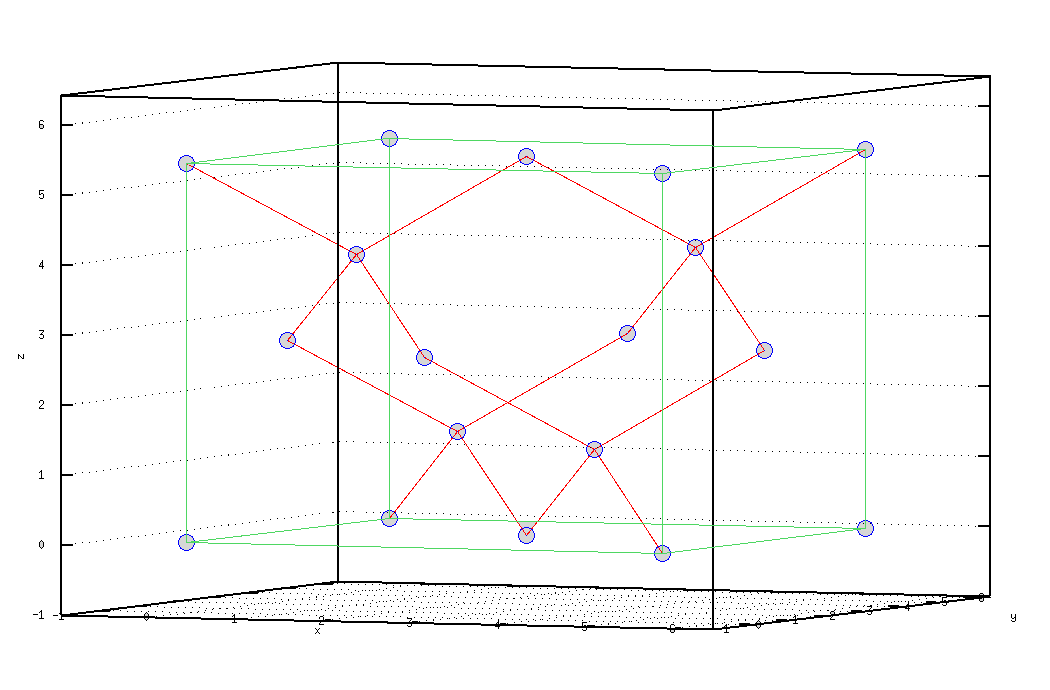
\includegraphics[scale=0.25]{img/si}
\end{center}
\end{frame}

\begin{frame}
\frametitle{GNN - learning algorithm}
\begin{enumerate}
	\item initialize randomly $h_w$ and $g_w$ weights
	\item until stop criterion is satisfied:
	\begin{itemize}
		\item random initialization of representation $X$
		\item FORWARD : calculate $X = F_w(X)$ until fixed point is reached
		\item BACKWARD : calculate $G_w(X)$ and backpropagate the error
		\item update $f_w$ and $g_w$ weights
	\end{itemize}
\end{enumerate}
\end{frame}

\begin{frame}
\frametitle{Forward - building representation}
\begin{columns}
	\begin{column}{0.66\textwidth}
		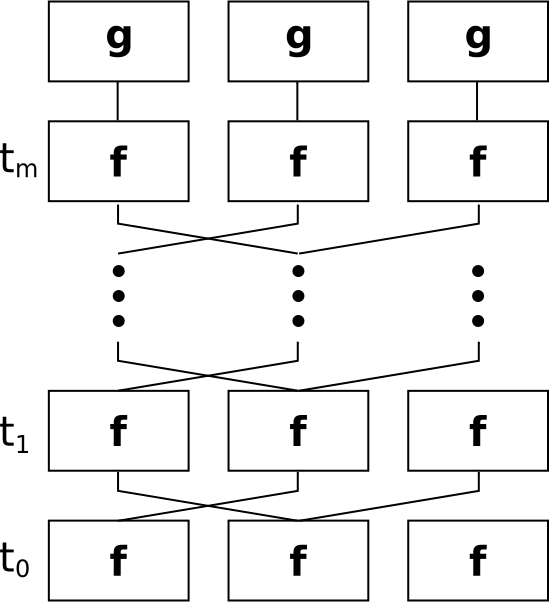
\includegraphics[scale=0.4]{img/forward2}
	\end{column}
	\begin{column}{0.34\textwidth}
		\begin{itemize}
			\item unfolding
		\end{itemize}
	\end{column}
\end{columns}
\end{frame}

\begin{frame}
\frametitle{Backward - backpropagation}
\begin{columns}
	\begin{column}{0.66\textwidth}
		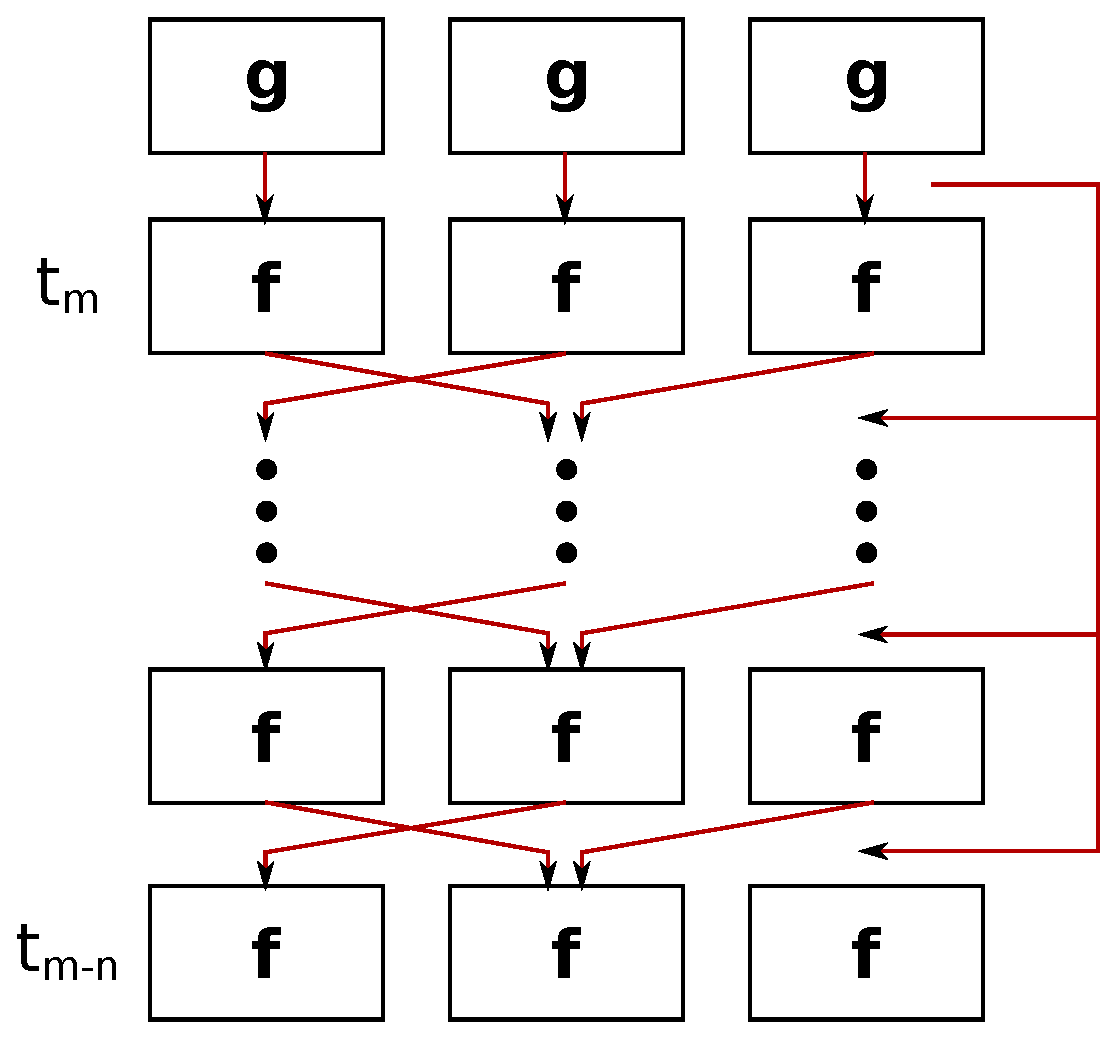
\includegraphics[scale=0.4]{img/backward2}
	\end{column}
	\begin{column}{0.34\textwidth}
		\begin{itemize}
			\item BPTT
			\item Almeida-Pineda
		\end{itemize}
	\end{column}
\end{columns}
\end{frame}

\begin{frame}
\frametitle{How do we know $F_w$ will reach fixed point?}
\begin{itemize}
	\item contraction map (Banach theorem)
	\item $||F_w(X_1) - F_w(X_2)|| \leq ||X_1 - X_2||$
	\item unique fixed point
	\item fixed point reached from every starting point
	\item very few iterations needed
	\item penalty imposed on $F_w$ weights when the contraction is lost
\end{itemize}
\end{frame}

\begin{frame}
\frametitle{How strong should the penalty be?}
\begin{center}
	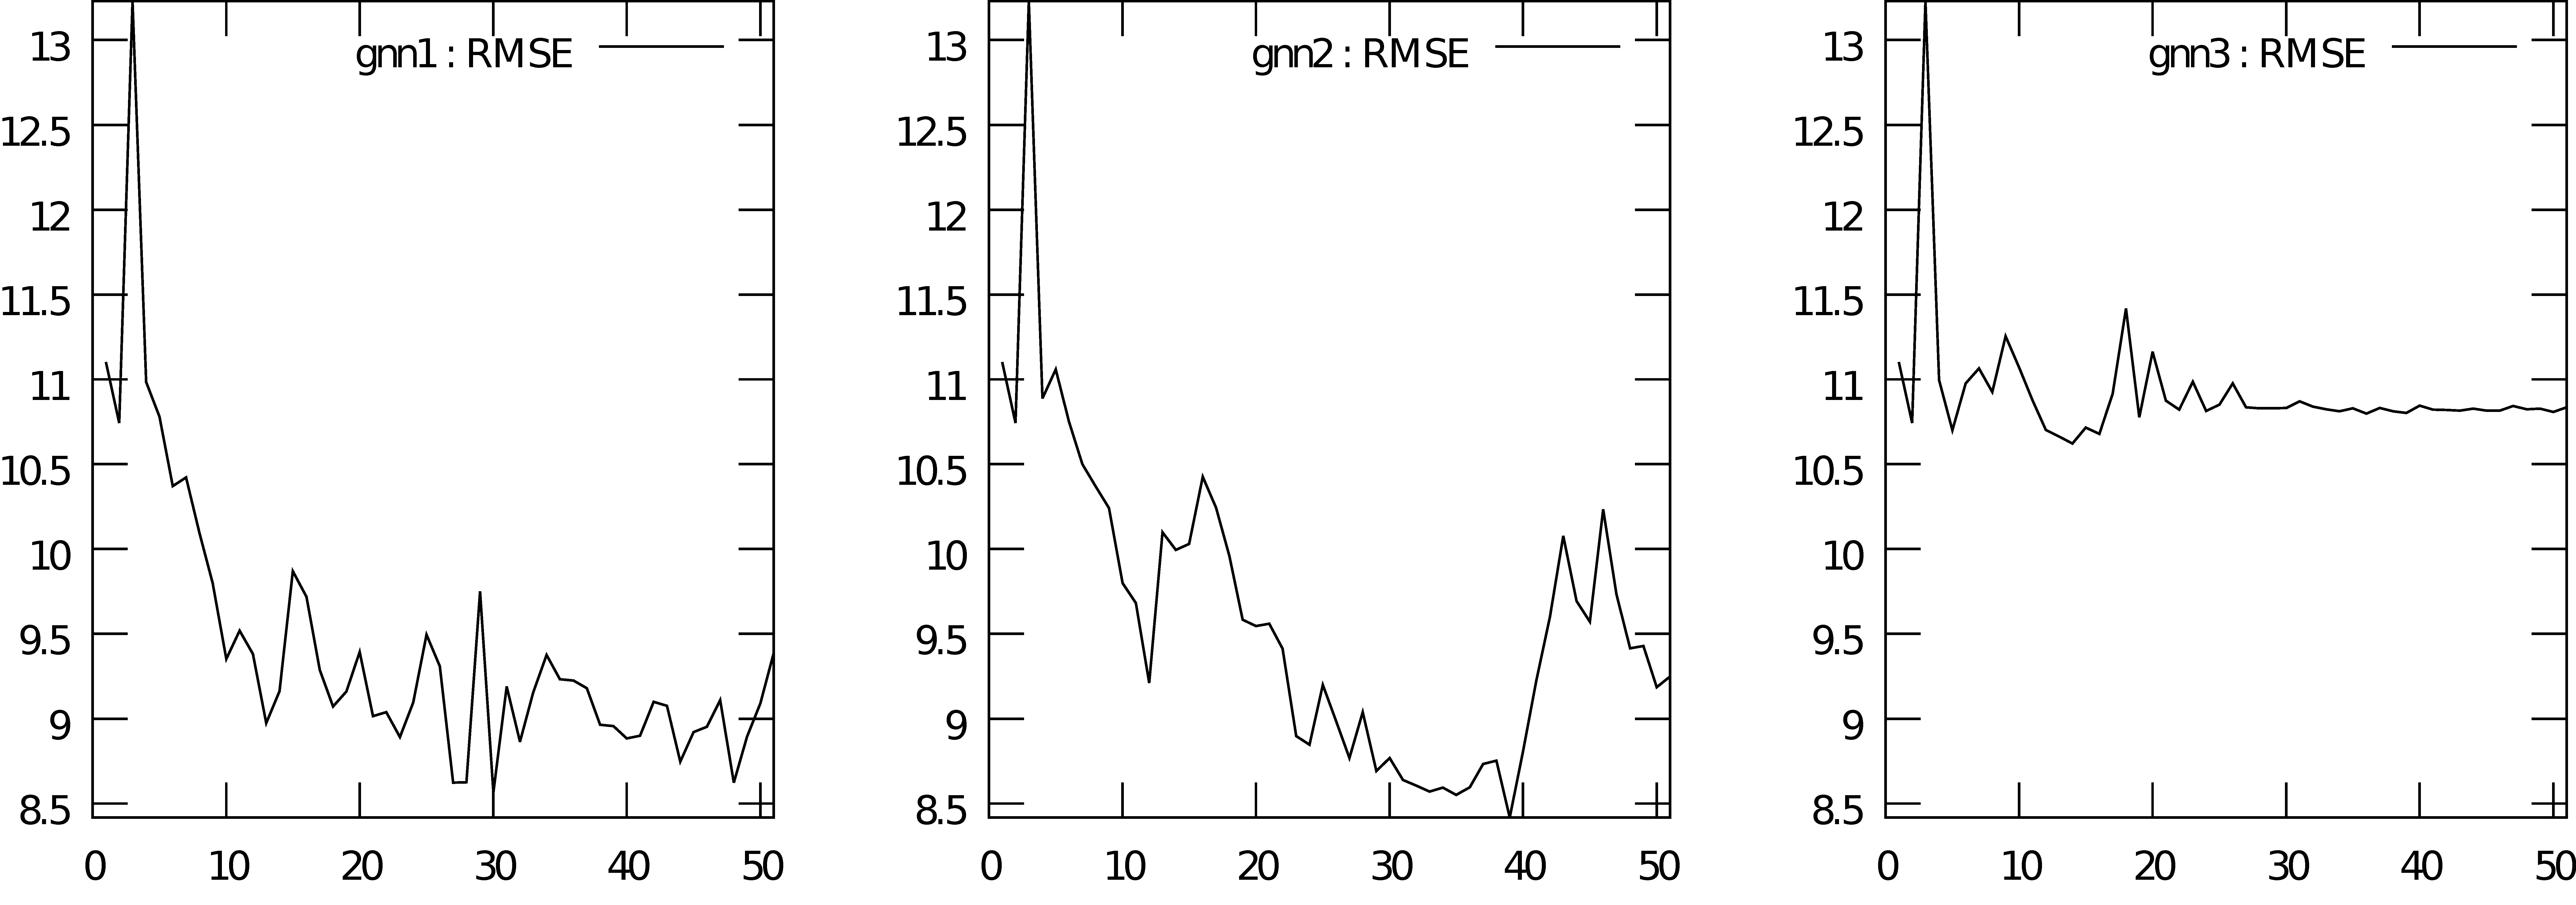
\includegraphics[scale=0.065]{img/rmse1_clipped}
\end{center}
\begin{itemize}
	\item $contractionConstant \in [1.2, 0.9, 0.6]$
	\item boundary value depends on dataset
\end{itemize}
\end{frame}

\end{document}
